\documentclass[11pt,a4paper]{article}

\usepackage[margin=2.3cm]{geometry}
\usepackage[T1]{fontenc}
\usepackage{lmodern}
\usepackage{microtype}
\usepackage{amsmath,amssymb}
\usepackage{graphicx}
\usepackage{booktabs}
\usepackage{caption}
\usepackage{float}
\usepackage[colorlinks=true,linkcolor=black,citecolor=black,urlcolor=blue]{hyperref}
\usepackage[version=4]{mhchem}
\usepackage{siunitx}

\graphicspath{{../figures/}}
\captionsetup{font=small,labelfont=bf}
\setlength{\parskip}{3pt}
\renewcommand{\topfraction}{0.9}
\renewcommand{\textfraction}{0.08}
\renewcommand{\floatpagefraction}{0.85}

\newcommand{\CH}{\ce{CH4}}
\newcommand{\OH}{\ce{OH}}

\title{\textbf{Why Is Methane Rising Again?}\\[2pt]
\large A Methane--OH Box Model of Recent Trends and the Global Methane Pledge}
\author{Shardul Junagade (23110297)\\[2pt]
\small EH-605 Modeling Earth System and Sustainability, IIT Gandhinagar\\
\small Instructor: Prof.\ R.\ N.\ Singh\\[2pt]
\small Final project report}
\date{14th November 2026}

\begin{document}
\maketitle

\begin{abstract}
\noindent
Atmospheric methane has been measured continuously since 1983. Its growth rate fell almost to zero between 2000 and 2006, rose again from 2007, and reached 15--18\,ppb\,yr$^{-1}$ in 2020--21, the highest in the record. In this project I fitted a series of box models to the NOAA global mean record for 1984--2025 to find out which processes are needed to reproduce these changes.

A one-box model with a constant lifetime of about 9 years misses the observations by 21\,ppb (RMS) and shows no stall. I then added the reaction of methane with \OH\ using mass-action kinetics. Because \OH\ adjusts within about a second, the two-variable system reduces to one equation in which the methane sink saturates like a Michaelis--Menten term. This feedback raises the lifetime of a methane perturbation from 9.3 to 12.7 years, and the system has a single stable equilibrium at any realistic emission rate. Adding the feedback by itself increased the error to 32\,ppb. The error dropped to 3\,ppb (7\,ppb on held-out years) once \OH\ was also allowed to depend on NOx and CO emissions and on temperature. In this model, rising NOx accounts for part of the 2000--06 stall, and the fall in NOx during COVID accounts for roughly half of the 2020--21 surge. I then ran the fitted model under future emission scenarios together with a two-layer energy-balance model. Meeting the Global Methane Pledge lowers methane in 2050 by about 330\,ppb and avoids about 0.05\,K of warming from methane's direct forcing. An optimal-control problem solved with GEKKO gives an optimal cut of about 35\,\% for a social cost of methane of \$1600 per tonne, close to the pledge's 30\,\%.
\end{abstract}

\section{Introduction}

Methane (\CH) is the second most important greenhouse gas made by people. Its concentration has risen from about 729\,ppb before industrialisation to 1936\,ppb in 2025, and its radiative forcing today is about \SI{0.57}{W.m^{-2}}, roughly a quarter of that of \ce{CO2}. Unlike \ce{CO2}, methane does not stay in the air for centuries. It is destroyed mainly by the hydroxyl radical (\OH) in the troposphere, which gives it a lifetime of about a decade. This short lifetime makes methane attractive for policy, because cutting emissions should show up in the atmosphere within a few years. That idea is behind the Global Methane Pledge, signed in 2021, which aims to cut anthropogenic methane emissions by 30\,\% from 2020 levels by 2030.

The same short lifetime makes the observed record hard to read. The growth rate of methane (Fig.~\ref{fig:record}) has gone through three surprising changes:
\begin{itemize}\itemsep0pt
\item a near standstill from 2000 to 2006;
\item a restart in 2007;
\item an unusually fast rise in 2020--21, during the pandemic, when human activity dropped.
\end{itemize}
Emission inventories show no pause in 2000--06; if anything they grow fastest then. So either the inventories are missing something, or the sink is changing. The sink also depends on methane itself, because the reaction with methane uses up \OH. More methane therefore means less \OH\ and a longer methane lifetime, a positive feedback similar to the ice--albedo feedback.

In this project I used box models, mass-action kinetics, stability analysis, an energy-balance model and dynamic optimisation to study this record. I started with a one-box model and added processes one at a time (the \OH\ feedback, then the effects of NOx, CO and temperature on \OH). I kept a process only if it improved the fit to the observations and the prediction of years left out of the fit.

\begin{figure}[t]
\centering
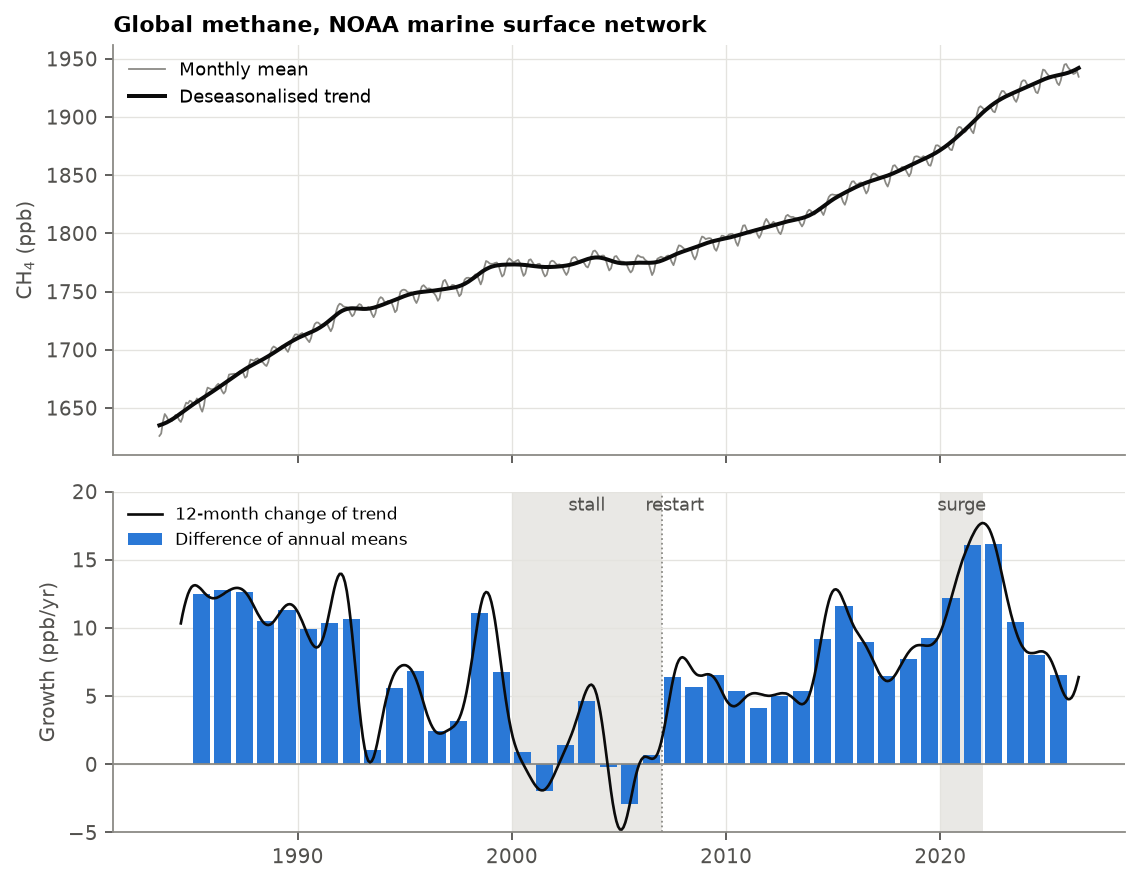
\includegraphics[width=0.6\linewidth]{01_record_growth.png}
\caption{Global mean methane from the NOAA marine surface network (top) and its growth rate (bottom). The stall, restart and surge that motivate this project are marked.}
\label{fig:record}
\end{figure}

\section{Objectives}

The project had three objectives, the same as in the project outline:
\begin{enumerate}\itemsep2pt
\item \textbf{Test the one-box model.} Find out whether a one-box model with a constant lifetime can reproduce the observed methane record since 1984, and if it cannot, why not.
\item \textbf{Analyse the methane--OH system and explain the growth rate.} Build a coupled methane--\OH\ model, study its equilibria, stability, feedback strength and possible tipping point, and find which processes explain the stall, the restart and the 2020 surge.
\item \textbf{Evaluate the Global Methane Pledge.} Estimate how much the pledge would lower methane concentration and warming by 2050, compared with the usual emission scenarios, and compare the pledge with an economically optimal abatement path.
\end{enumerate}

\section{Data}

All data are public. They were downloaded by a script that also checks each file for coverage, value ranges and agreement between overlapping sources (Table~\ref{tab:data}). All code is available at \url{https://github.com/ShardulJunagade/methane-oh-box-model}, and the whole analysis reruns with \texttt{uv run scripts/run\_all.py}.

\begin{table}[h]
\centering\small
\caption{Datasets used.}
\label{tab:data}
\begin{tabular}{p{6.0cm}p{2.6cm}p{6.0cm}}
\toprule
Dataset & Period & Used for\\
\midrule
NOAA GML global mean \CH\ (doi:10.15138/P8XG-AA10) & 1983--2025 & target of every model fit\\
EDGAR 2025 \CH\ emissions (Crippa et al., 2025) & 1970--2024 & anthropogenic emissions\\
CEDS + fires (Indicators of Global Climate Change) & 1970--2025 & second inventory; NOx and CO emissions\\
Indicators of Global Climate Change, ERF & 1750--2025 & forcing check, total forcing\\
Global Carbon Project budget (Saunois et al., 2025) & 2000--2020 & independent budget check\\
HadCRUT5 global temperature & 1850--2025 & energy-balance calibration\\
RCMIP SSP emissions and concentrations & to 2100 & future scenarios\\
\bottomrule
\end{tabular}
\end{table}

Two properties of the data matter for what follows. First, the inventories disagree: EDGAR gives 333\,Tg\,yr$^{-1}$ of anthropogenic methane for 2024, while CEDS with fires gives 368. Second, the inventories grow fastest during the stall. EDGAR grows by 3.9\,Tg\,yr$^{-2}$ during 2000--06 but only 2.8\,Tg\,yr$^{-2}$ during 2007--19, the opposite of what the concentrations do. I convert between mass and mixing ratio with $\beta=\SI{2.75}{Tg}$ per ppb, the methane analogue of the 2.123\,GtC per ppm used for \ce{CO2}.

\section{Methodology}

\subsection{Overall approach}
I first wrote down the simplest models (a one-box model, then the \CH--\OH\ kinetic system) and analysed them on paper: equilibria, stability and time scales. I then fitted a hierarchy of increasingly detailed versions to the observed record, keeping a new process only if it improved both the fit and the out-of-sample prediction. Finally, the best model was coupled to an energy-balance model and run into the future under different emission scenarios, including the pledge, and used to find an optimal abatement path.

Everything was written in Python. The box models were integrated with a fourth-order Runge--Kutta scheme with monthly steps (error against the analytic solution: 0.08\,ppb), the full, stiff \CH--\OH\ system with an implicit (Radau) solver, and the fits used SciPy's \texttt{least\_squares}.

\subsection{One-box model and mass balance}
The simplest description treats the atmosphere as one well-mixed box:
\begin{equation}
\frac{dC}{dt}=\frac{E_a(t)+E_n}{\beta}-\frac{C}{\tau},
\label{eq:onebox}
\end{equation}
where $C$ is the global mean mixing ratio, $E_a$ the anthropogenic emissions from EDGAR, $E_n$ a constant natural source and $\tau$ the lifetime. For exponentially growing emissions $E_a=q\,e^{\alpha t}$ it has the closed-form solution
\begin{equation}
C(t)=C_0e^{-t/\tau}+\frac{E_n\tau}{\beta}\left(1-e^{-t/\tau}\right)+\frac{q/\beta}{\alpha+1/\tau}\left(e^{\alpha t}-e^{-t/\tau}\right),
\end{equation}
which I used to check the numerical solver. Turned around, the same equation gives the total emissions implied by the observations,
\begin{equation}
E(t)=\beta\left(\frac{dC}{dt}+\frac{C}{\tau}\right),
\label{eq:topdown}
\end{equation}
without any inventory, with $dC/dt$ from centred differences of the annual means.

\subsection{Methane and OH as a kinetic system}
By the law of mass action, the reaction $\ce{CH4 + OH -> products}$ proceeds at a rate proportional to $[\CH][\OH]$. Writing $X$ for \OH\ relative to its 2010 value, a minimal two-variable system is
\begin{align}
\frac{dC}{dt}&=\frac{E}{\beta}-k\,X\,C-k_oC, \label{eq:ch4}\\
\frac{dX}{dt}&=\frac{1}{\tau_X}\Big[P-X\Big(a\frac{C}{C_r}+1-a\Big)\Big], \label{eq:oh}
\end{align}
where $P$ is the \OH\ production and the other parameters are listed in Table~\ref{tab:params}. The bracket says that \OH\ is destroyed partly by methane (a share $a$) and partly by other gases, mainly CO.

\OH\ lives about one second ($\tau_X\approx\SI{1}{s}$), so it settles almost at once. Setting $dX/dt=0$ gives a single equation with a saturating sink,
\begin{equation}
S(C)=\frac{k\,C}{a\,C/C_r+1-a}+k_oC,
\label{eq:sink}
\end{equation}
which has the same shape as the Michaelis--Menten (Monod) uptake law. Two lifetimes follow from it: the global lifetime $\tau=C/S(C)$ and the perturbation lifetime $\tau_p=1/S'(C)$, which controls how fast an extra pulse of methane decays (from linear stability analysis). Their ratio $f=\tau_p/\tau$ is the feedback factor. The equilibria for a given emission rate solve $E/\beta=S(C)$, and their stability follows from the Jacobian of Eqs.~\eqref{eq:ch4}--\eqref{eq:oh}.

\begin{table}[t]
\centering\small
\caption{Model parameters. Fitted values are from the best model (V4), with one standard error; the others are fixed from published studies or from the observations.}
\label{tab:params}
\begin{tabular}{llll}
\toprule
Symbol & Meaning & Value & Source\\
\midrule
$\beta$ & Tg of \CH\ per ppb & 2.75 & \href{https://doi.org/10.5194/essd-17-1873-2025}{literature}\\
$1/k$ & \CH\ lifetime against \OH\ (prior) & $11.2\pm1.3$\,yr & \href{https://doi.org/10.1029/2012GL051440}{literature}\\
$k$ & \OH\ loss frequency of \CH & $0.098\pm0.004$\,yr$^{-1}$ & fitted\\
$k_o$ & stratosphere, soil and Cl sinks & 0.020\,yr$^{-1}$ & \href{https://doi.org/10.1029/2012GL051440}{literature}\\
$a$ & share of \OH\ loss due to \CH & 0.31 & \href{https://doi.org/10.5194/acp-13-285-2013}{literature}\\
$C_r$ & reference \CH\ (2010) & 1799\,ppb & observed\\
$E_n$ & natural + non-inventory source & $306\pm19$\,Tg\,yr$^{-1}$ & fitted\\
$g_N$, $g_C$ & \OH\ sensitivity to NOx, CO emissions & $0.33\pm0.02$, $0.19\pm0.02$ & fitted\\
$E_a/R$ & activation temperature of \CH+\OH & 1775\,K & \href{https://ntrs.nasa.gov/citations/20210006316}{literature}\\
$C$ & upper-layer heat capacity & 16.7\,W\,yr\,m$^{-2}$\,K$^{-1}$ & fitted\\
$\lambda$ & climate feedback parameter & 1.25\,W\,m$^{-2}$\,K$^{-1}$ & fitted\\
$\gamma$, $C_d$ & deep-ocean coupling and heat capacity & 0.67, 100 (same units) & \href{https://doi.org/10.1175/JCLI-D-12-00195.1}{literature}\\
\bottomrule
\end{tabular}
\end{table}

\subsection{Model hierarchy, fitting and evaluation}
I fitted increasingly detailed versions of Eq.~\eqref{eq:ch4}, with \OH\ in steady state, to the NOAA annual means for 1984--2025.
\begin{itemize}\itemsep0pt
\item \textbf{V1:} constant lifetime (Eq.~\ref{eq:onebox}).
\item \textbf{V2:} adds the \CH--\OH\ feedback (Eq.~\ref{eq:sink}).
\item \textbf{V3:} also lets \OH\ production depend on NOx and CO emissions:
\[P=\left(\frac{E_{\mathrm{NOx}}}{E_{\mathrm{NOx},r}}\right)^{g_N}\left(\frac{E_{\mathrm{CO}}}{E_{\mathrm{CO},r}}\right)^{-g_C}.\]
\item \textbf{V4:} additionally lets the rate constant follow the Arrhenius law with the observed temperature anomaly, $k\propto \exp(1775\,\Delta T/T^2)$ with $T=272$\,K.
\end{itemize}
The parameters $\theta$ were found by minimising
\begin{equation}
J(\theta)=\sum_{i}\left(\frac{C_{\mathrm{model},i}-C_{\mathrm{obs},i}}{\sigma}\right)^2+\left(\frac{k-k_0}{\sigma_k}\right)^2,
\end{equation}
with $\sigma=3$\,ppb. The second term is needed because the lifetime and the natural source trade off against each other (Section~\ref{sec:onebox}), so the data alone cannot fix both. I therefore added the literature value $1/k_0=11.2\pm1.3$\,yr (Prather et al., 2012) as a soft constraint. Parameter standard errors come from the Jacobian of the residuals at the optimum.

Models were compared by the RMS error, by the Akaike information criterion, $\mathrm{AIC}=n\ln(\mathrm{RSS}/n)+2p$, which penalises the number of parameters $p$, and by a holdout test (fit to 1984--2012 only, then predict 2013--2025). To attribute the three events, I re-ran the best model with one driver (anthropogenic emissions, NOx, CO or temperature) held at its value from the year before the event, and measured how much the mean growth rate changed.

\subsection{Forcing, warming and scenarios}
Methane forcing was computed with the simple square-root formula $0.036(\sqrt{M}-\sqrt{M_0})$ and with the formula used in IPCC AR6, and compared with the official series. Warming was computed with a zero-dimensional energy-balance model extended by a deep-ocean layer, that is, a two-box model for heat:
\begin{equation}
C\frac{dT}{dt}=F-\lambda T-\gamma(T-T_d),\qquad C_d\frac{dT_d}{dt}=\gamma(T-T_d).
\label{eq:ebm}
\end{equation}
$C$ and $\lambda$ were fitted to the HadCRUT5 anomalies (relative to 1850--1900) using the total forcing since 1750; $\gamma$ and $C_d$ were taken from the literature.

For the future, the best model was driven by the SSP scenarios (their methane, NOx and CO emissions relative to 2025, and the IPCC AR6 warming of each scenario), by the pledge path (a linear cut to 70\,\% of the 2020 level by 2030, then held), and by two limiting cases: emissions frozen at 2025, and all anthropogenic emissions stopped. Warming differences were computed with Eq.~\eqref{eq:ebm}. Uncertainty in the pledge result was estimated from 200 Monte Carlo runs, each drawing the fitted parameters from their covariance, $a$ from 0.25--0.37 and $\lambda$ from $1.25\pm0.25$.

\subsection{Optimal abatement}
To ask whether a 30\,\% cut is the right size, I posed abatement as an optimal-control problem, in the same way as the classic optimal fishery-harvest problem. The control $u(t)\in[0,0.7]$ is the fraction of baseline (SSP2-4.5) anthropogenic emissions $E_b$ removed in year $t$, and the best-fit model gives the resulting concentration $C$. Abatement costs $\tfrac12 m u^2E_b$ per year with $m=\$4000$\,t$^{-1}$, so that the marginal cost rises linearly with $u$. Two problems were solved:
\begin{itemize}\itemsep0pt
\item \textbf{Problem A (cost--benefit)} weighs abatement costs against climate damage,
\begin{equation}
\min_u\ \sum_{t=2025}^{2100} e^{-rt}\Big[\tfrac12 m\,u^2E_b+D\,C\Big],\qquad r=2\,\%\,\text{yr}^{-1},
\end{equation}
where $D$ is chosen so that one tonne emitted today costs the social cost of methane (\$800, \$1600 or \$3200 per tonne).
\item \textbf{Problem B (target)} finds the cheapest path that reaches the pledge's 2050 concentration and stays below it afterwards.
\end{itemize}
Both were solved with GEKKO in its dynamic-optimisation mode (IMODE 6, IPOPT solver) on an annual grid. For Problem A the optimum can also be estimated by hand: marginal cost equals marginal damage when $u^*\approx\mathrm{SC}/m$.

\section{Analysis and results}

\subsection{One-box model}
\label{sec:onebox}
With the lifetime fixed at 9.15\,yr, the one-box model misses the observations by 21\,ppb RMS (Fig.~\ref{fig:onebox}). It also shows no stall, because it keeps rising through 2000--06 along with the EDGAR emissions. When the model is fitted only to 1984--2005 and run forward, it overshoots 2025 by 39\,ppb. If the lifetime is left free, the fit improves to 12.6\,ppb, but only by shrinking the lifetime to 6.4\,yr and pushing the natural source to 500\,Tg\,yr$^{-1}$. Both values are physically unrealistic. The misfit surface explains why: the error has a long, narrow valley along which a shorter lifetime is traded for a larger natural source, so the data alone cannot pin down both. This is the reason the later fits carry a prior on the lifetime.

\begin{figure}[t]
\centering
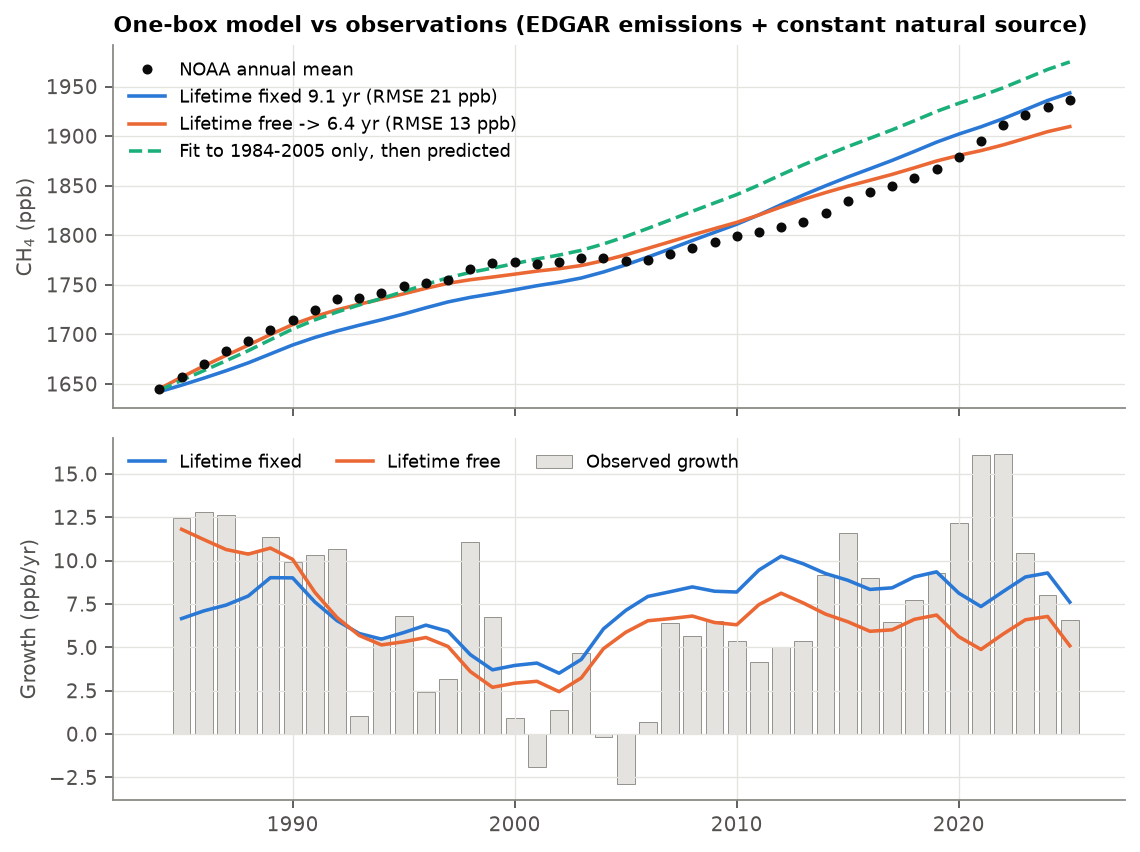
\includegraphics[width=0.56\linewidth]{02_one_box_fit.png}\hfill
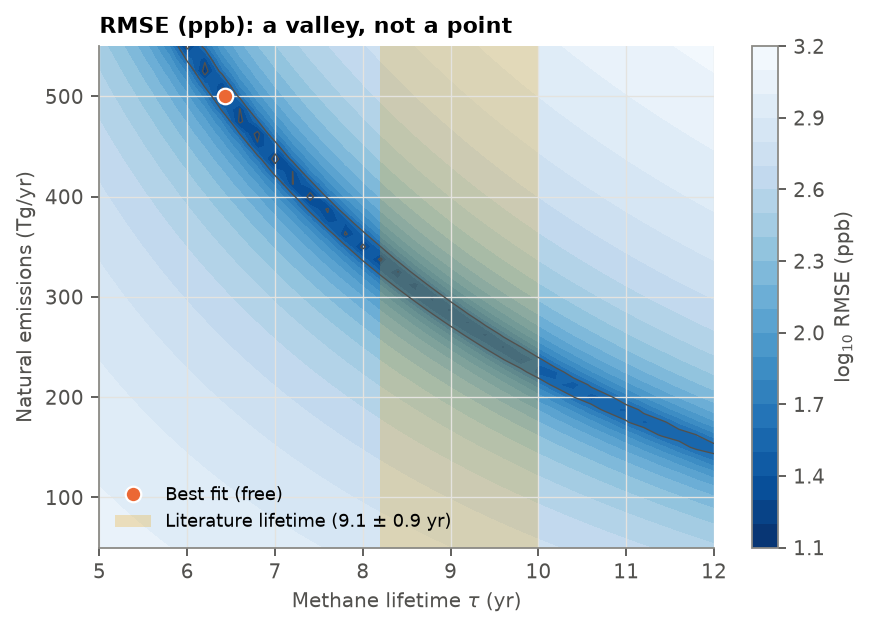
\includegraphics[width=0.42\linewidth]{02_cost_surface.png}
\caption{Left: the one-box model against observations, with fixed and free lifetime, and a run fitted only to 1984--2005. Right: RMS error as a function of lifetime and natural emissions. The low-error region is a long, narrow valley; the yellow band is the lifetime known from independent studies.}
\label{fig:onebox}
\end{figure}

The same equation can also be used in reverse (Eq.~\ref{eq:topdown}) to estimate total emissions from the observations. With $\tau=9.1$\,yr, the observed record implies total emissions of 574\,Tg\,yr$^{-1}$ for 2010--19, almost identical to the Global Carbon Project's independent estimate of 575\,Tg\,yr$^{-1}$. The part not covered by EDGAR (natural sources plus whatever the inventory misses) was 289\,Tg\,yr$^{-1}$ in 1985--99, 268 in 2000--06, 267 in 2007--19 and 291 in 2020--22. It dropped by about 20\,Tg\,yr$^{-1}$ during the stall and rose by about 25 in the surge, which the later fits come back to.

\subsection{The methane--OH feedback}
At today's state, the Jacobian of Eqs.~\eqref{eq:ch4}--\eqref{eq:oh} has two eigenvalues: $-3.2\times10^{7}$\,yr$^{-1}$ (a time scale of 0.98\,s, for \OH) and $-0.079$\,yr$^{-1}$ (12.7\,yr, for methane). The system is extremely stiff, and replacing it by the reduced Eq.~\eqref{eq:sink} changes the solution by only $4\times10^{-6}$\,ppb. The phase portrait (Fig.~\ref{fig:oh}, right) shows this fast--slow structure directly: trajectories drop almost vertically onto the \OH\ nullcline and then creep along it towards a single stable node.

The feedback lengthens the response time. In 2025 the global lifetime is 9.33\,yr but the perturbation lifetime is 12.69\,yr, a feedback factor of $f=1.36$, inside the 1.3--1.4 range quoted in the literature. A 100\,Tg pulse decays with an e-folding time of 12.7\,yr with feedback and 9.2\,yr without, consistent with the eigenvalue. Methane itself has already lowered \OH\ by about 2\,\% since 2010.

\begin{figure}[t]
\centering
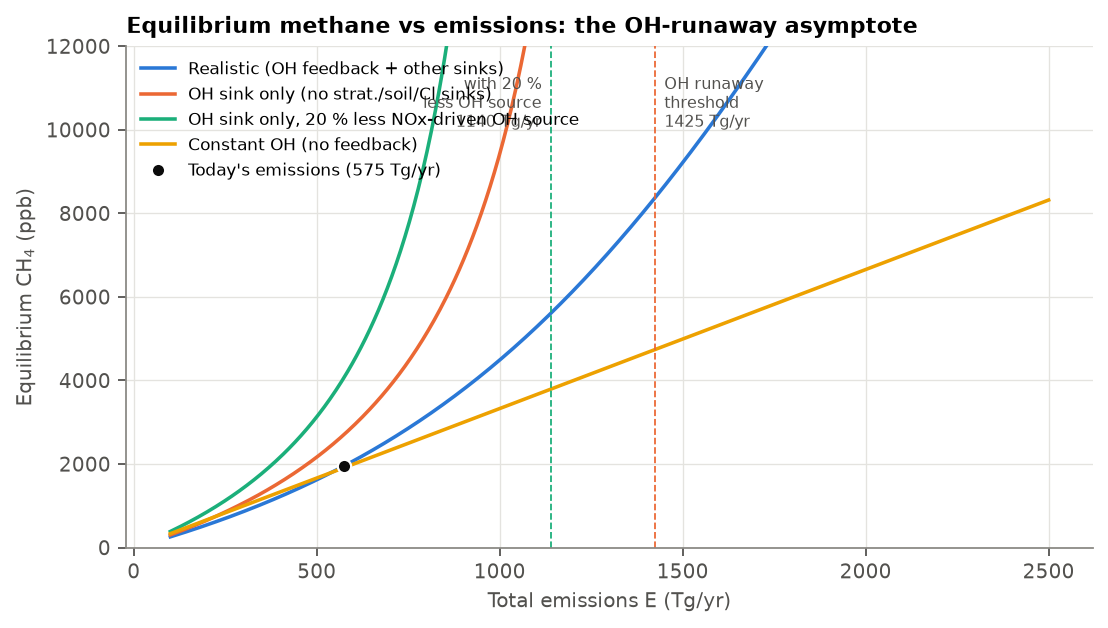
\includegraphics[width=0.49\linewidth]{03_equilibrium_threshold.png}\hfill
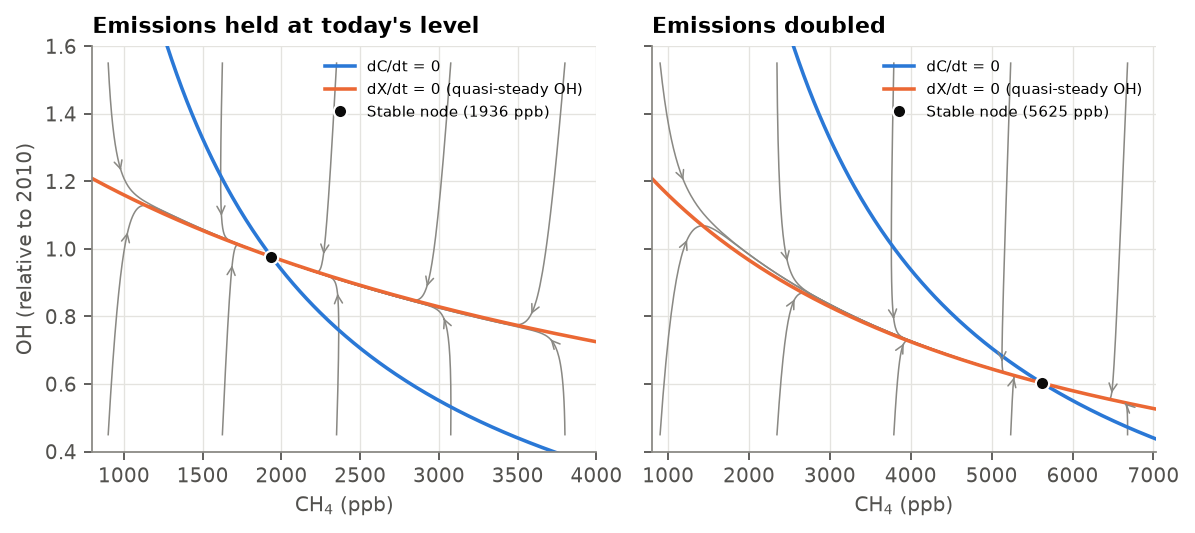
\includegraphics[width=0.49\linewidth]{03_phase_portrait.png}
\caption{Left: equilibrium methane as a function of total emissions. With \OH\ as the only sink, equilibrium is lost at 1425\,Tg\,yr$^{-1}$ (dashed); the other sinks remove this asymptote. Right: phase portraits for today's emissions and for doubled emissions (\OH\ slowed artificially to make the fast step visible).}
\label{fig:oh}
\end{figure}

Is there a tipping point? Because $S(C)$ increases monotonically, there is exactly one stable equilibrium for any emission rate, with no bistability and no hysteresis, unlike the snowball-Earth energy-balance model. If \OH\ were the only sink, though, the saturation in Eq.~\eqref{eq:sink} would cap removal at $\beta kC_r/a$, and above
\begin{equation}
E_{\mathrm{crit}}=\frac{\beta\,k\,C_r}{a}\approx\SI{1425}{Tg.yr^{-1}}
\end{equation}
no equilibrium would exist at all. That is about 2.5 times today's emissions, and it drops to 1140\,Tg\,yr$^{-1}$ if the \OH\ source falls by 20\,\%. The slower, non-saturating sinks ($k_oC$) remove the singularity: equilibrium methane then rises steeply with emissions but stays finite. Holding today's 575\,Tg\,yr$^{-1}$ forever would bring methane to about 1955\,ppb, only slightly above today's level.

\subsection{What explains the stall, restart and surge}
Table~\ref{tab:models} and Fig.~\ref{fig:fits} compare the model hierarchy. Adding the \CH--\OH\ feedback alone (V2) increased the RMS error from 21 to 32\,ppb. The feedback amplifies the response to rising emissions, so the modelled growth during 2000--06 became even larger. The fit improved only when \OH\ was allowed to respond to processes outside the methane cycle. With NOx and CO emissions as drivers (V3) the error drops to 3.1\,ppb. With the temperature dependence of the rate constant added (V4) the AIC is lowest, and V4 also predicts the held-out years 2013--25 best (6.7\,ppb).

\begin{table}[t]
\centering\small
\caption{Model hierarchy fitted to NOAA annual means, 1984--2025. ``Growth $r$'' is the correlation of modelled and observed annual growth; ``holdout'' is the RMS error for 2013--25 when fitted to 1984--2012 only.}
\label{tab:models}
\setlength{\tabcolsep}{4.5pt}
\begin{tabular}{lcccccc}
\toprule
Model & Params & $\tau$ (yr) & RMS (ppb) & AIC & Growth $r$ & Holdout (ppb)\\
\midrule
V1 one-box, lifetime fixed & 1 & 9.15 & 21.0 & 257.8 & 0.37 & 34.7\\
V1$'$ one-box, lifetime free & 2 & 6.43 & 12.6 & 216.8 & 0.48 & 17.6\\
V2 + \CH--\OH\ feedback & 1 & 9.15 & 32.2 & 293.5 & 0.20 & 62.6\\
V3 + NOx and CO drivers & 4 & 7.59 & 3.1 & 102.9 & 0.79 & 14.2\\
\textbf{V4 + Arrhenius temperature} & 4 & \textbf{8.47} & \textbf{3.0} & \textbf{100.1} & \textbf{0.80} & \textbf{6.7}\\
\bottomrule
\end{tabular}
\end{table}

\begin{figure}[t]
\centering
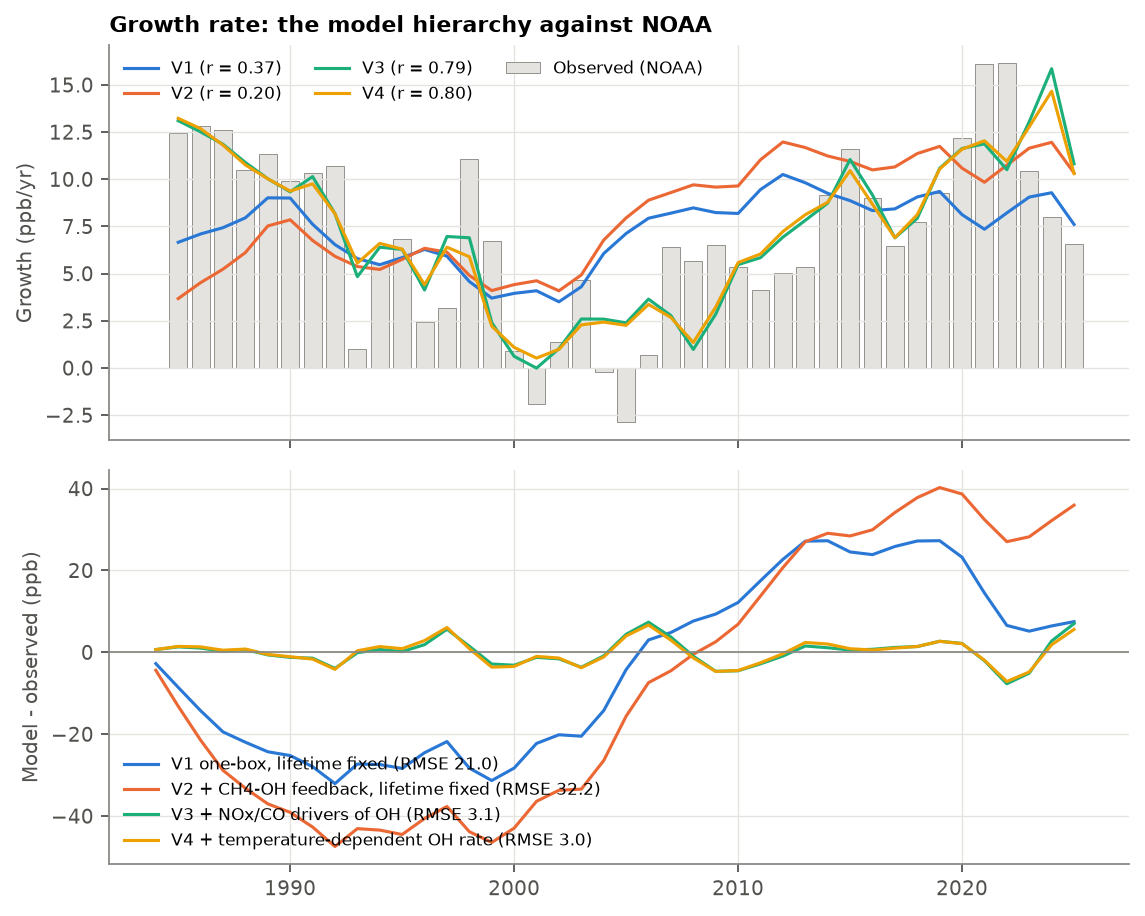
\includegraphics[width=0.55\linewidth]{04_model_hierarchy.png}\hfill
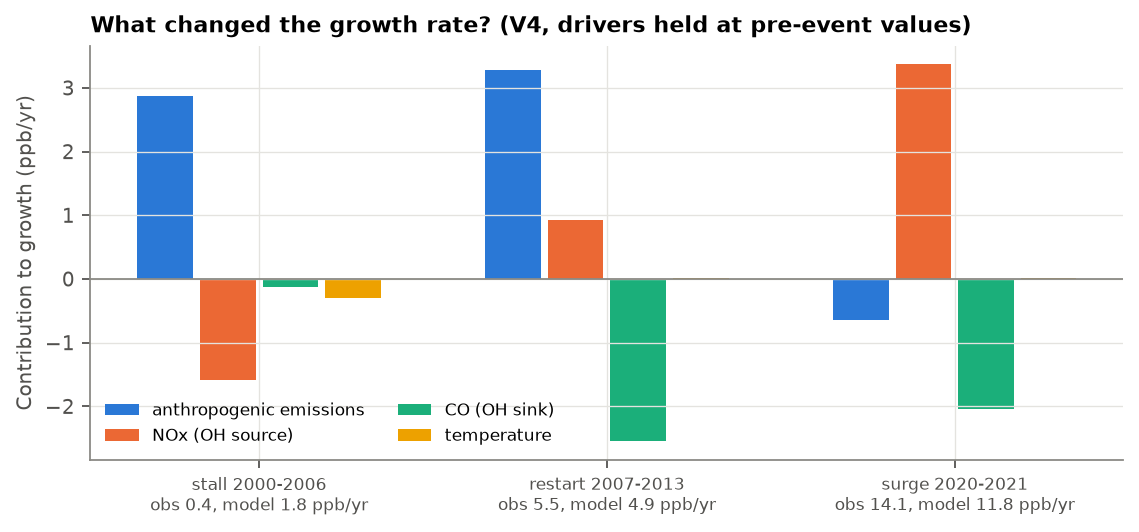
\includegraphics[width=0.44\linewidth]{04_attribution.png}
\caption{Left: modelled and observed growth rates (top) and residuals (bottom) for the model hierarchy. Right: contribution of each driver to the growth rate in the three periods, from runs with that driver held at its pre-event value.}
\label{fig:fits}
\end{figure}

The fitted sensitivities are $g_N=0.33\pm0.02$ and $g_C=0.19\pm0.02$. The value of $g_N$ is probably larger than a chemistry model would give, so I read it as an effective sensitivity that may also absorb other trends correlated with NOx. Swapping EDGAR for the CEDS inventory changes the error by less than 0.3\,ppb. Fitting the feedback strength $a$ as well gives $0.07\pm0.14$; the concentration record cannot determine it, which is why the literature value is used.

Holding one driver fixed at a time (Fig.~\ref{fig:fits}, right) gives the following picture.
\begin{itemize}\itemsep0pt
\item \textbf{Stall (2000--06).} Inventory growth alone would have added about 2.9\,ppb\,yr$^{-1}$. Model \OH\ was about 3\,\% higher than in the late 1990s, mostly because NOx emissions rose, and this removed 1.6\,ppb\,yr$^{-1}$. The model still gives 1.8\,ppb\,yr$^{-1}$ against the observed 0.4. Together with the dip in non-inventory emissions found above, this suggests that natural or unaccounted emissions also fell during the stall.
\item \textbf{Restart (2007--13).} NOx emissions peaked around 2006 and \OH\ stopped rising, while emissions kept growing.
\item \textbf{Surge (2020--21).} The pandemic drop in NOx added 3.4\,ppb\,yr$^{-1}$, and lower CO emissions took away 2.0\,ppb\,yr$^{-1}$. The model reaches 11.8\,ppb\,yr$^{-1}$ against the observed 14.1, and the remaining gap fits the extra 25\,Tg\,yr$^{-1}$ found in the mass balance.
\end{itemize}
The surge result can be checked against an independent study. Stevenson et al.\ (2022) used sensitivities from full chemistry models and found that the lockdown cut in NOx raised methane growth by 4.8\,ppb\,yr$^{-1}$ and the cut in CO lowered it by 1.4\,ppb\,yr$^{-1}$, enough to explain over half of the 2020 increase. My model gives the same signs and similar magnitudes (+3.4 and $-2.0$\,ppb\,yr$^{-1}$).

\subsection{Forcing and warming}
The square-root formula gives 0.61\,W\,m$^{-2}$ of methane forcing for 2025, about 7\,\% above the official 0.57\,W\,m$^{-2}$, because it ignores the overlap between methane and \ce{N2O} absorption bands. The AR6 formula matches the official series to 0.002\,W\,m$^{-2}$ over 1750--2025 and is used from here on.

Fitted to HadCRUT5, the two-layer model of Eq.~\eqref{eq:ebm} gives $\lambda=1.25$\,W\,m$^{-2}$\,K$^{-1}$, close to the commonly used Budyko value $B=1.3$, and an equilibrium climate sensitivity of 3.1\,K. The one-layer model fits the same record with $\lambda=1.78$ (sensitivity 2.2\,K), because it treats heat taken up by the deep ocean as if it were a radiative feedback. The two-layer model warms by 1.50\,K by 2025 (observed 1.43\,K), of which methane's direct forcing is responsible for 0.28\,K, about a fifth.


\subsection{Futures and the Global Methane Pledge}
Driven by the SSP scenarios, the model gives the methane paths in Fig.~\ref{fig:scen} and Table~\ref{tab:scen}. Its SSP2-4.5 projection (2005\,ppb in 2050, 1759\,ppb in 2100) is close to that of MAGICC7, the emulator used in IPCC assessments (2020 and 1683\,ppb). If all anthropogenic emissions stopped, methane would decay with an e-folding time of 9.9\,yr towards about 835\,ppb.

\begin{figure}[!htb]
\centering
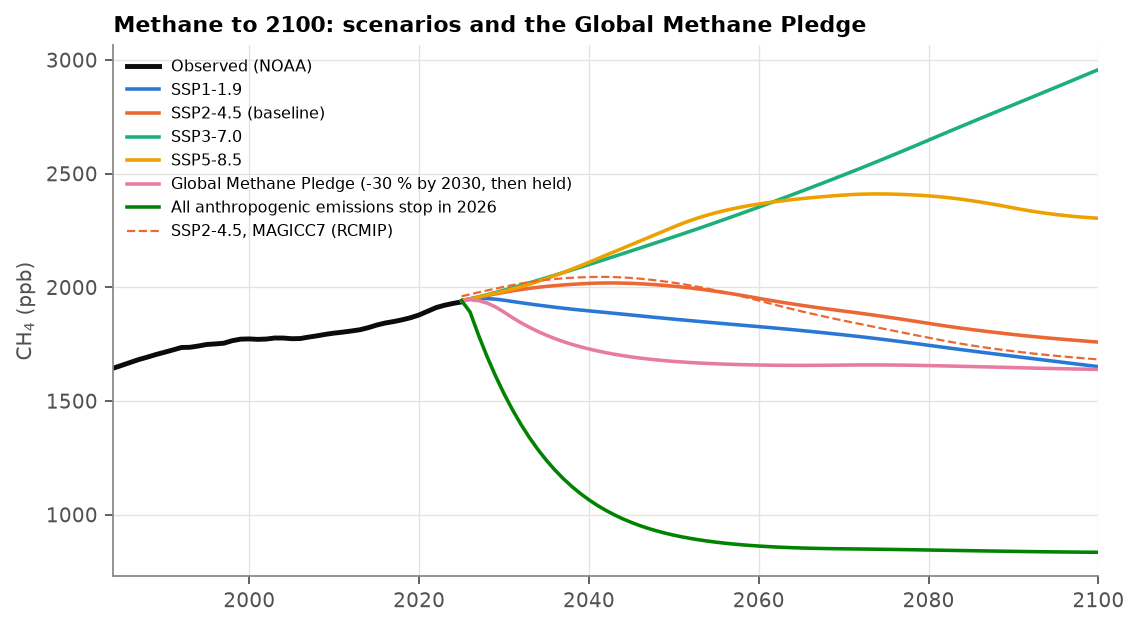
\includegraphics[width=0.62\linewidth]{07_scenarios.png}
\caption{Projected methane for several scenarios and for the Global Methane Pledge, with the MAGICC7 projection for SSP2-4.5 (dashed) as a check.}
\label{fig:scen}
\end{figure}

\begin{table}[!htb]
\centering\small
\caption{Methane (ppb) and warming relative to SSP2-4.5 for selected futures.}
\label{tab:scen}
\begin{tabular}{lcccc}
\toprule
Scenario & 2030 & 2050 & 2100 & $\Delta T_{2050}$ (K)\\
\midrule
SSP1-1.9 & 1943 & 1860 & 1651 & $-0.022$\\
SSP2-4.5 (baseline) & 1978 & 2005 & 1759 & 0\\
SSP5-8.5 & 1983 & 2266 & 2304 & $+0.026$\\
Global Methane Pledge & 1891 & 1674 & 1639 & $-0.054$\\
Emissions frozen at 2025 & 1974 & 2061 & 2095 & $+0.004$\\
All anthropogenic emissions stop & 1532 & 910 & 835 & $-0.206$\\
\bottomrule
\end{tabular}
\end{table}

The pledge lowers methane in 2050 by 333\,ppb (5--95\,\% range 310--352) compared with SSP2-4.5, and avoids 0.055\,K (0.047--0.065\,K) of warming through methane's direct forcing. The pledge's own claim of at least 0.2\,K by 2050 is larger, mainly because it counts methane's indirect effects through ozone and other routes, which this model leaves out. Because methane lives about a decade, the benefit appears quickly, but it also disappears quickly if the cuts are not maintained: the pledge path levels off after 2040 instead of continuing to fall.

\subsection{Optimal abatement}
In the cost--benefit problem (Fig.~\ref{fig:opt}), GEKKO finds a nearly constant abatement fraction, set where the marginal cost of abatement equals the damage caused by one more tonne. For a social cost of methane of \$800, \$1600 and \$3200 per tonne, the 2030 abatement is 19, 36 and 68\,\%, close to the hand estimates of 20, 40 and 70\,\% (the last one capped). At \$1600\,t$^{-1}$, close to the central US EPA (2023) estimate, the optimum of about 35\,\% is close to the pledge's 30\,\%. Abatement drops towards zero near 2100, because cuts made at the end of the horizon no longer have time to pay off. This is the same end effect seen in optimal fishery-harvest problems.

The target problem gives a very different path. To reach the pledge's 2050 concentration as cheaply as possible, the optimiser delays: it abates only 7\,\% in 2030 and builds up to a spike of 54\,\% just before 2050. Early cuts would have mostly decayed by the deadline, and later spending is discounted. The pledge path costs 1.5 times as much for the same 2050 level (present value \$1271 vs \$855 billion), but it keeps methane lower throughout the 2030s and 2040s. With a target for a single date, the cheapest strategy is to act at the last minute, so a target based on cumulative methane, or the cost--benefit approach above, would give steadier cuts.

\begin{figure}[!htb]
\centering
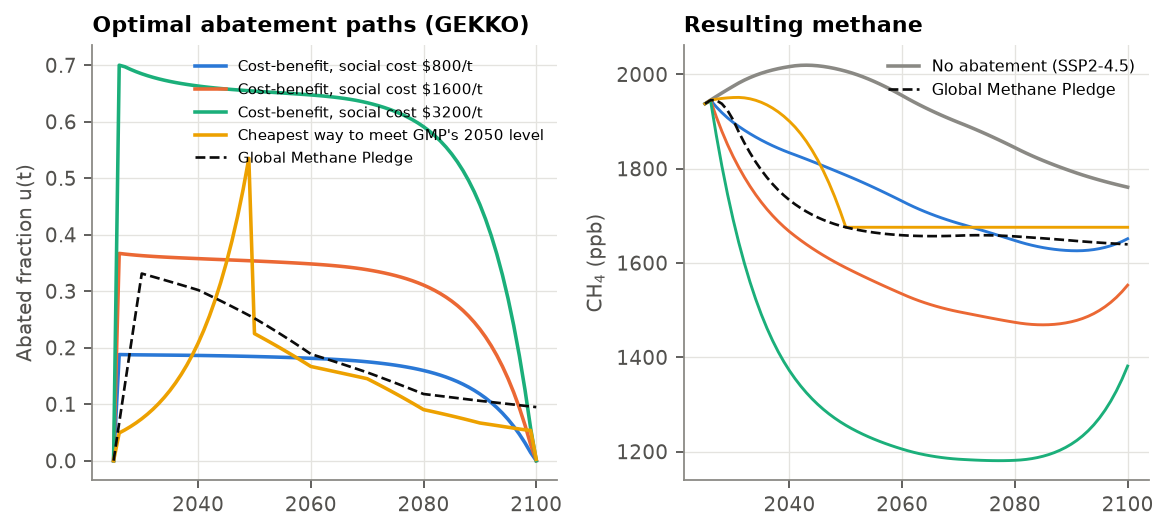
\includegraphics[width=0.74\linewidth]{08_optimal_abatement.png}
\caption{Optimal abatement paths from GEKKO for three values of the social cost of methane (SC) and for the cheapest path to the pledge's 2050 level, compared with the pledge (left), and the resulting methane (right).}
\label{fig:opt}
\end{figure}

\section{Limitations}
The models use one global box with annual means, so there is no seasonal cycle and no spatial structure in \OH, and the CO--\OH\ chemistry enters only through an effective exponent. The fitted NOx sensitivity probably soaks up other effects, so the attribution to NOx should be read as indicative. Natural emissions are held constant, although real wetland emissions vary with rainfall and El Ni\~no; this is why the model under-predicts the 2020--22 surge. The warming estimates include only methane's direct forcing, and the abatement cost curve is illustrative, so the shapes of the optimal paths are more reliable than the dollar figures. A natural next step would be a three-box \CH--CO--\OH\ model, in which CO is a variable rather than an emission input.

\section{Key findings}
\begin{enumerate}\itemsep2pt
\item \textbf{The one-box model fails with a realistic lifetime.} With a lifetime of 9.15\,yr the model misses the record by 21\,ppb RMS and shows no stall. It fits reasonably only with a lifetime of 6.4\,yr, which is too short. Used in reverse as a mass balance, the same model gives total emissions of 574\,Tg\,yr$^{-1}$ for 2010--19, within 1\,Tg\,yr$^{-1}$ of the Global Carbon Project estimate.
\item \textbf{The methane--OH feedback lengthens the lifetime but does not produce the stall.} Because methane uses up \OH, a perturbation decays over 12.7\,yr instead of 9.3\,yr (feedback factor 1.36). Adding this feedback raised the model error from 21 to 32\,ppb.
\item \textbf{There is no tipping point at realistic emissions.} With \OH\ as the only sink, no equilibrium would exist above 1425\,Tg\,yr$^{-1}$, about 2.5 times today's emissions. The other sinks (stratosphere, soil, chlorine) remove this limit, leaving one stable equilibrium.
\item \textbf{Changes in OH driven by NOx, CO and temperature explain most of the record.} With them the model fits 1984--2025 to within 3\,ppb. Rising NOx removed 1.6\,ppb\,yr$^{-1}$ during the stall, and the fall in NOx during COVID added 3.4\,ppb\,yr$^{-1}$ in 2020--21, about half of the surge, in agreement with Stevenson et al.\ (2022). Roughly 25\,Tg\,yr$^{-1}$ of extra emissions is still needed to explain the full surge.
\item \textbf{The pledge acts quickly, but its effect is modest.} It lowers methane by about 330\,ppb and warming by about 0.05\,K by 2050 through direct forcing, and the benefit stops when the cuts stop. For a social cost of \$1600 per tonne the optimal cut is about 35\,\%, close to the pledge's 30\,\%. With only a 2050 target, the cheapest path delays most cuts until the late 2040s.
\end{enumerate}

\small
\begin{thebibliography}{9}\itemsep0pt
\bibitem{crippa} Crippa, M.\ et al.\ (2025). \emph{GHG emissions of all world countries -- 2025 report}. EU Joint Research Centre (EDGAR).
\bibitem{ipcc} IPCC (2021). \emph{Climate Change 2021: The Physical Science Basis}. Contribution of Working Group I to the Sixth Assessment Report. Cambridge University Press.
\bibitem{prather} Prather, M.\,J., Holmes, C.\,D., Hsu, J.\ (2012). Reactive greenhouse gas scenarios: systematic exploration of uncertainties and the role of atmospheric chemistry. \emph{Geophys.\ Res.\ Lett.} 39, L09803.
\bibitem{saunois} Saunois, M.\ et al.\ (2025). Global Methane Budget 2000--2020. \emph{Earth Syst.\ Sci.\ Data} 17, 1873--1958.
\bibitem{stevenson} Stevenson, D.\,S., Derwent, R.\,G., Wild, O., Collins, W.\,J.\ (2022). COVID-19 lockdown emission reductions have the potential to explain over half of the coincident increase in global atmospheric methane. \emph{Atmos.\ Chem.\ Phys.} 22, 14243--14252, doi:10.5194/acp-22-14243-2022.
\bibitem{epa} US EPA (2023). \emph{Report on the Social Cost of Greenhouse Gases: Estimates Incorporating Recent Scientific Advances}. U.S. Environmental Protection Agency, Washington, DC.
\end{thebibliography}

\end{document}
